Many types of self-propelled microorganisms moving through water tend to accummulate near the boundaries
of their environments. This has been observed both experimentally, \cite{rothschild1963non}, 
\cite{berke2008hydrodynamic} and in nature. Figure \ref{fig:both_images} shows two characteristic
illustrations of this behaviour by plotting the density cells and bacteria observed cross-sectionally 
within their domains.

\begin{figure}[htbp]\label{fig: intro_distributions}
    \centering
    \begin{subfigure}[b]{0.45\textwidth}
      \centering
      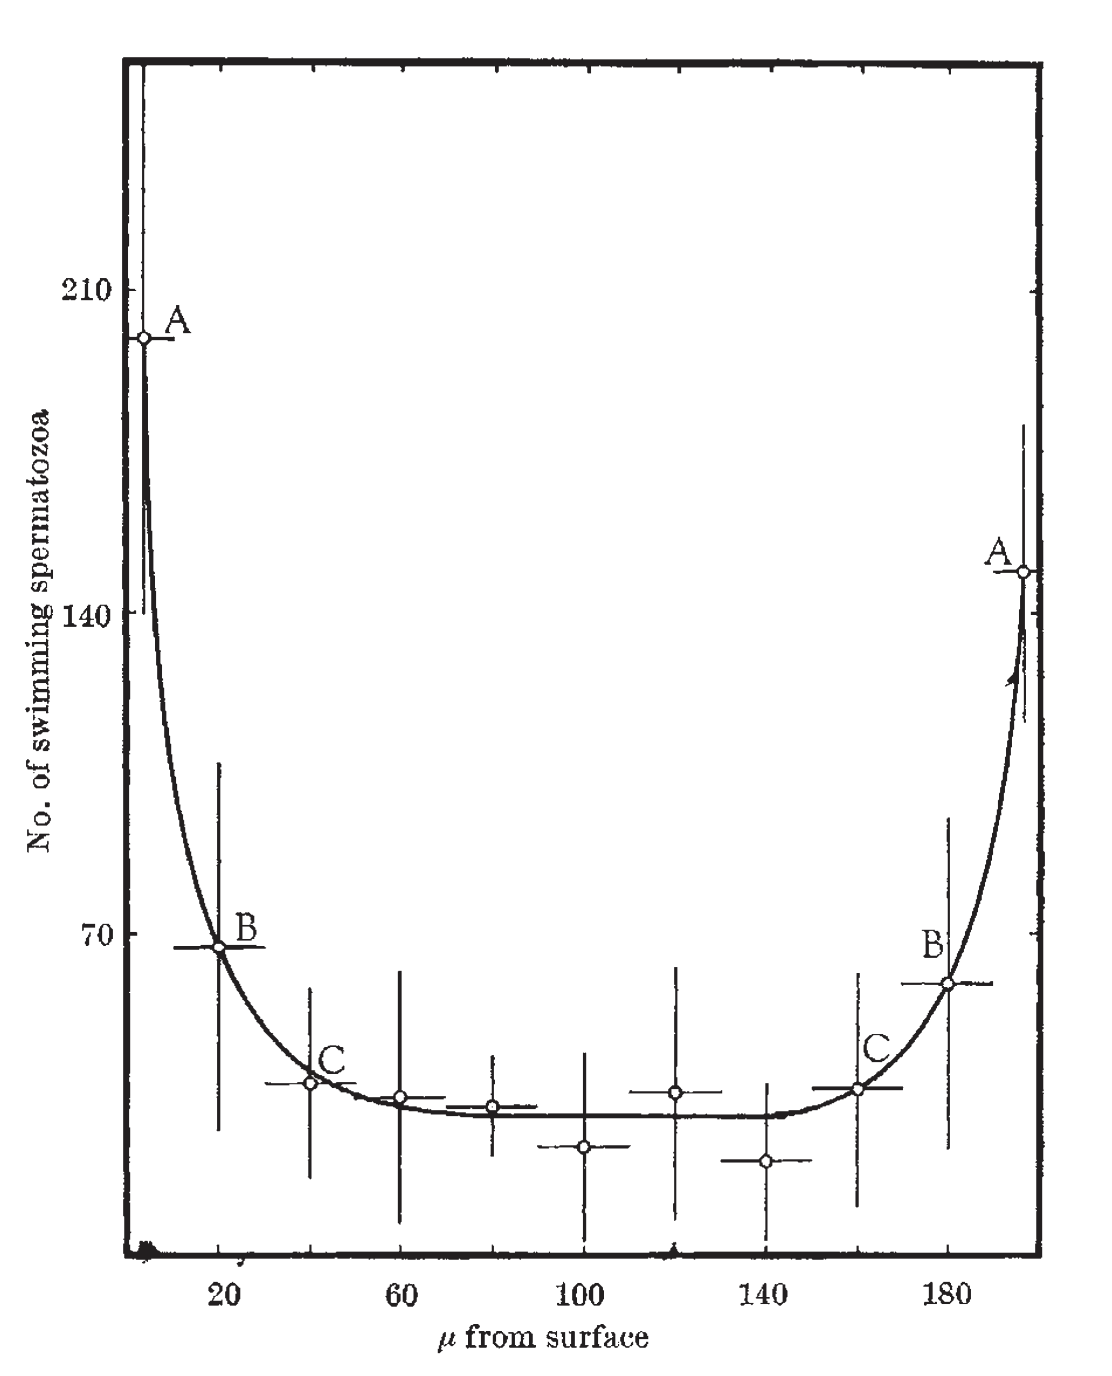
\includegraphics[width=\textwidth]{graphics/bull_spermatazoa_ distribution.png}
      \caption{Distribution of bull spermatazoa in suspended medium \cite{rothschild1963non}.}
      \label{fig:image1}
    \end{subfigure}
    \hfill
    \begin{subfigure}[b]{0.45\textwidth}
      \centering
      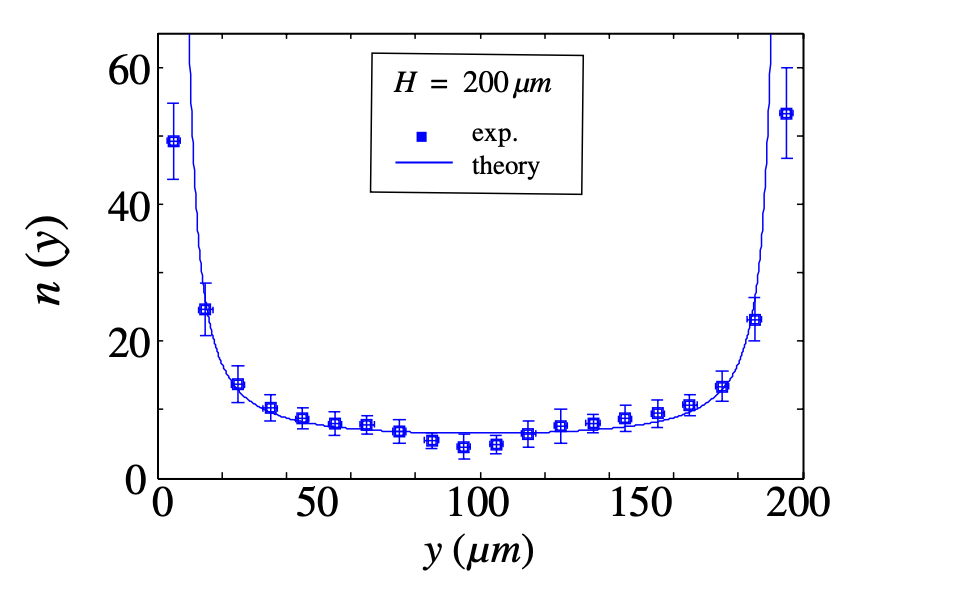
\includegraphics[width=\textwidth]{graphics/e_coli_distribution.png}
      \caption{Distribution of E. coli bacteria between two glass plate \cite{berke2008hydrodynamic}.}
      \label{fig:image2}
    \end{subfigure}
    \caption{Experimental results illustrating boundary accummulation of swimming microorganisms.}
    \label{fig:both_images}
  \end{figure}

Many models have been proposed to describe the behaviour of microswimmers(\cite{chen2021shape},
\cite{berke2008hydrodynamic}, \cite{ai2013rectification}), and this observed boundary accummulation is
an important feature for such models to capture. The purpose of such models is not only to describe this behaviour
but also to provide some explanation behind it.


The goal of this report is to present three models that describe the behaviour of swimming microorganisms,
with a particular focus on capturing the observed boundary accummulation. Before introducing these models, 
a brief overview of stochastic PDEs and the Fokker-Planck equation will be given.

The structure of this report is as follows:

